\section{SZ Compression Pipeline and Prediction Configurations}
\label{sec:background:pipeline}
\label{sec:baseline-configurations}

SZ3~\cite{zhao2021optimizing,liang2022sz3}, QoZ~\cite{liu2022dynamic,liu2024high}, and ASZ share an SZ-family compression pipeline and several prediction concepts. This section first describes the pipeline and defines the terminology used throughout the paper, then examines the prediction configurations in SZ3 and QoZ that are most directly relevant to ASZ.

\subsection{Pipeline Overview}

\begin{figure}[htb]
\centering
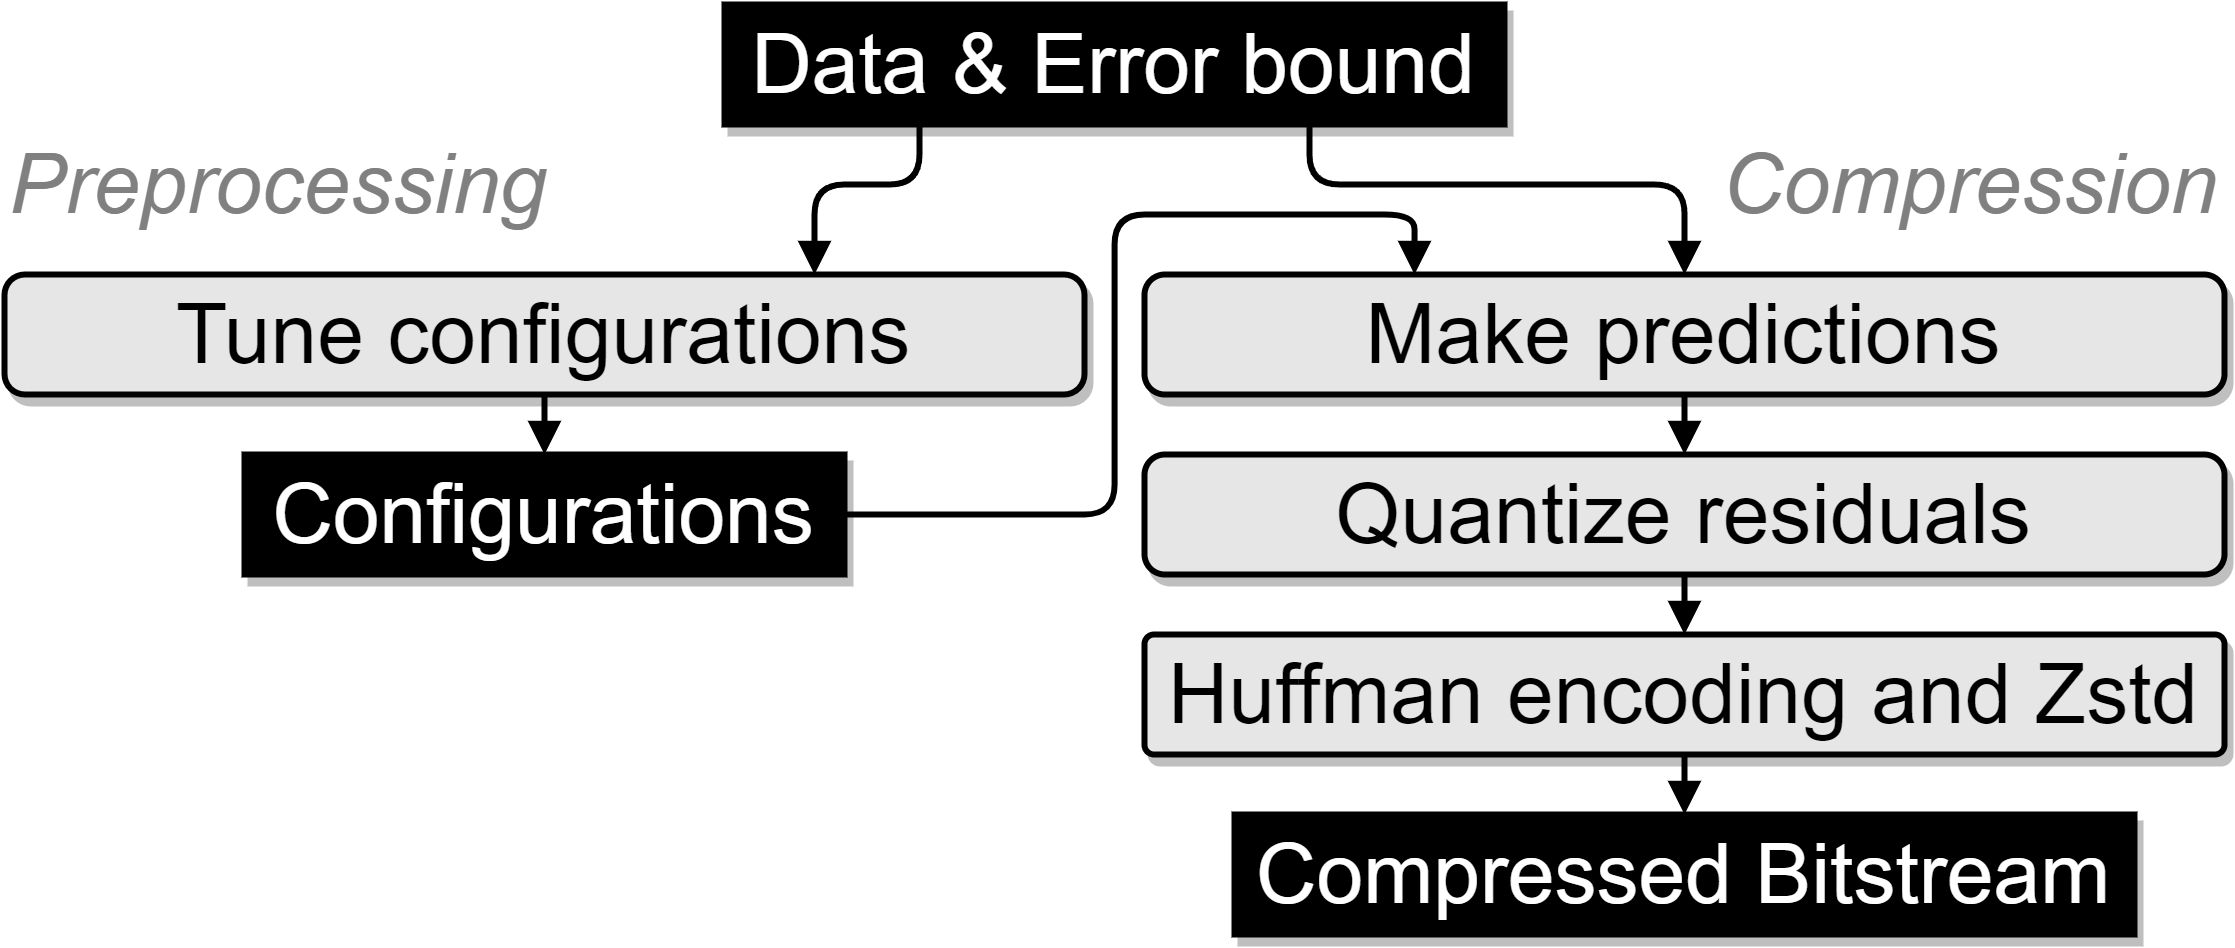
\includegraphics[width=.840909\columnwidth]{revised-fig/0-sz-diagram.png}
\caption{Overview of the SZ compression pipeline. Preprocessing selects a configuration that guides prediction during compression. The compressor quantizes prediction residuals and losslessly encodes the resulting QB indices using Huffman coding followed by Zstd.}
\label{fig:pipeline:sz}
\end{figure}

This pipeline comprises prediction, residual quantization, and lossless compression. Prediction and quantization alternate as the compressor traverses the data. Lossless compression processes the resulting QB indices after the traversal.

For each target value $x_i$, the predictor estimates it from $m$ previously reconstructed reference values:
\begin{equation}
\label{eq:background:prediction}
p_i=\sum_{j=1}^{m}w_j\hat x_{i,j},
\end{equation}
where $\hat x_{i,j}$ denotes the reconstructed value of the $j$th reference and $w_j$ is its weight.

The prediction residual $e_i=x_i-p_i$ is then quantized into an integer quantization-bin (QB) index $q_i$, from which the reconstructed value $\hat x_i$ is obtained:
\begin{equation}
\label{eq:background:quantization}
q_i=\operatorname{round}\!\left(\frac{e_i}{\Delta}\right),\qquad \hat x_i=p_i+\Delta\cdot q_i.
\end{equation}
Setting $\Delta\leq2\epsilon_{\mathrm{abs}}$ guarantees $|x_i-\hat x_i|\leq\epsilon_{\mathrm{abs}}$ in exact arithmetic.

These pointwise prediction and quantization operations are organized into a coarse-to-fine sequence of prediction rounds. SZ3, QoZ, and ASZ begin with a sparse set of available reference values. In each round, they predict and reconstruct a new subset of grid points, which then serve as references for later rounds. Consequently, the number of reconstructed points approximately doubles from one round to the next. Ignoring boundary effects, this progression means that the final round predicts $1/2$ of the field and the final three rounds together predict $7/8$.

After the final round, the QB indices are serialized in the selected order and compressed using Huffman coding followed by Zstd.

\subsection{Prediction Terminology}
\label{sec:pipeline:terminology}

This subsection defines the terminology used throughout the paper.

\begin{figure}[htb]
\centering
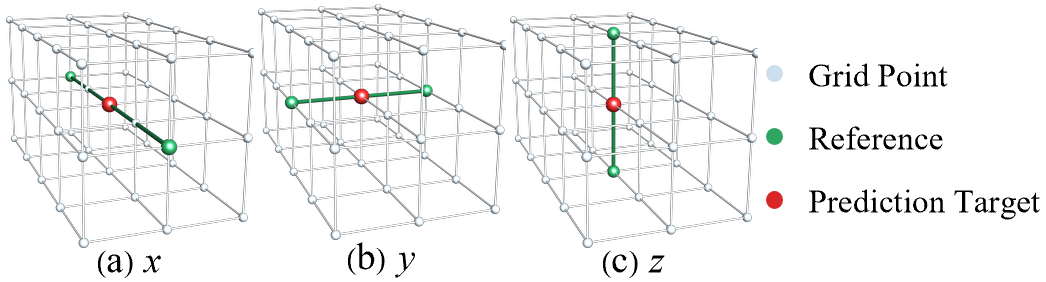
\includegraphics{../stencils_in_3_directions.png}
\caption{The same two-reference linear-interpolation stencil aligned with the three axes of a three-dimensional field.}
\label{fig:related-work:stencil-axes}
\end{figure}

\begin{enumerate}
\item \emph{Prediction Stencil.} A prediction stencil specifies the pattern of reference points around a target. In Fig.~\ref{fig:related-work:stencil-axes}, each predictor uses the same two-reference stencil, consisting of two collinear reconstructed points on opposite sides of the target.

\item \emph{Prediction Axis.} A prediction axis specifies how a stencil is oriented relative to the data grid and therefore which directional correlations it can exploit. The three predictors in Fig.~\ref{fig:related-work:stencil-axes} use the same stencil along different axes, reference different reconstructed points, and exploit different directional correlations.

\item \emph{Prediction Coefficients.} Prediction coefficients are the weights $w_j$ assigned to the references in Eq.~\eqref{eq:background:prediction}. Together with the stencil, they determine the prediction formula.

\item \emph{QB Serialization Order.} Before lossless compression, the QBs produced for multidimensional data must be written as a one-dimensional sequence. The serialization order determines whether QBs adjacent along the $x$-, $y$-, or $z$-axis appear consecutively in this sequence. Reordering preserves the QB values, their frequencies, and the reconstructed data, but changes the Huffman-codeword sequence presented to Zstd and can therefore affect lossless compression.

\item \emph{Configuration Granularity.} Configuration granularity specifies the scope over which a selected choice is shared, such as a field, a group of rounds, one round, or one data block.
\end{enumerate}
